\documentclass[../AnalysisNoteJBuxton.tex]{subfiles}
\begin{document}

%\subsection{Results: \texorpdfstring{$\Lambda$K$^{0}_{S}$ and $\Lambda$K$^{\pm}$}{TEXT}}
\subsection{Results: \LamKs and \LamKpm}
\label{ResultsLamK}

In the following sections, we present results assuming (i) no residual correlations (Sec. \ref{ResultsLamK_NoRes}), (ii) three residual contributors (Sec. \ref{ResultsLamK_3Res}), and (iii) ten residual contributors (Sec. \ref{ResultsLamK_10Res}).  We find the case of three and ten contributors to be consistent; therefore, for simplicity, we will quote the result utilizing three residuals as our final result.

For the results shown, unless otherwise noted, the following hold true:
All correlation functions were normalized in the range 0.32 $< k^{*} <$ 0.40 GeV/c, and fit in the range 0.0 $< k^{*} <$ 0.30 GeV/c.
For the \LamKchM and \ALamKchP analyses, the region 0.19 $< k^{*} <$ 0.23 GeV/$c$ was excluded from the fit to exclude the bump caused by the $\Omega^{-}$ resonance.
The non-femtoscopic background was modeled by a (6$^{\mathrm{th}}$-)order polynomial fit to THERMINATOR simulation.
The \LamKchPALamKchM radii are shared with \LamKchMALamKchP, while the \LamKsALamKs radii are unique.
In the figures showing experimental correlation functions with fits, the black solid line represents the primary (\LamK) correlation's contribution to the fit.
The green line shows the fit to the non-flat background.  
The purple points show the fit after all residuals' contributions have been included, and momentum resolution and non-flat background corrections have been applied.


Before beginning, I first collect a summary of my final results in Figure \ref{fig:ScattParams_Final}.  In the summary plot, we show the extracted scattering parameters in the form of a Im[f$_{0}$] vs Re[f$_{0}$] plot, which includes the d$_{0}$ values to the right side.  We also show the $\lambda$ vs. radius parameters for all three of our studied centrality bins.  In Fig. \ref{fig:ScattParams_Final}, three residual contributors were used, and the background was modeled by a (6$^{\mathrm{th}}$-)order polynomial fit to THERMINATOR simulation.  For the \LamKs results shown in the figure, the \LamKs and \ALamKs analyses were fit simultaneously across all centralities (0-10\%, 10-30\%, 30-50\%); scattering parameters and a single $\lambda$ parameter were shared amongst all, the radii were shared amongst results of like-centrality, and each has a unique normalization parameter.  For the \LamKpm results shown, all four pair combinations were fit simultaneously (\LamKchP, \ALamKchM, \LamKchM, \ALamKchP) across all centralities.  Scattering parameters were shared between pair-conjugate systems (i.e. a parameter set describing \LamKchP \& \ALamKchM, and a separate set describing \LamKchM \& \ALamKchP).  For each centrality, a radius and $\lambda$ parameters were shared between all pairs.  Each analysis has a unique normalization parameter.

\begin{figure}[h]
  \centering
  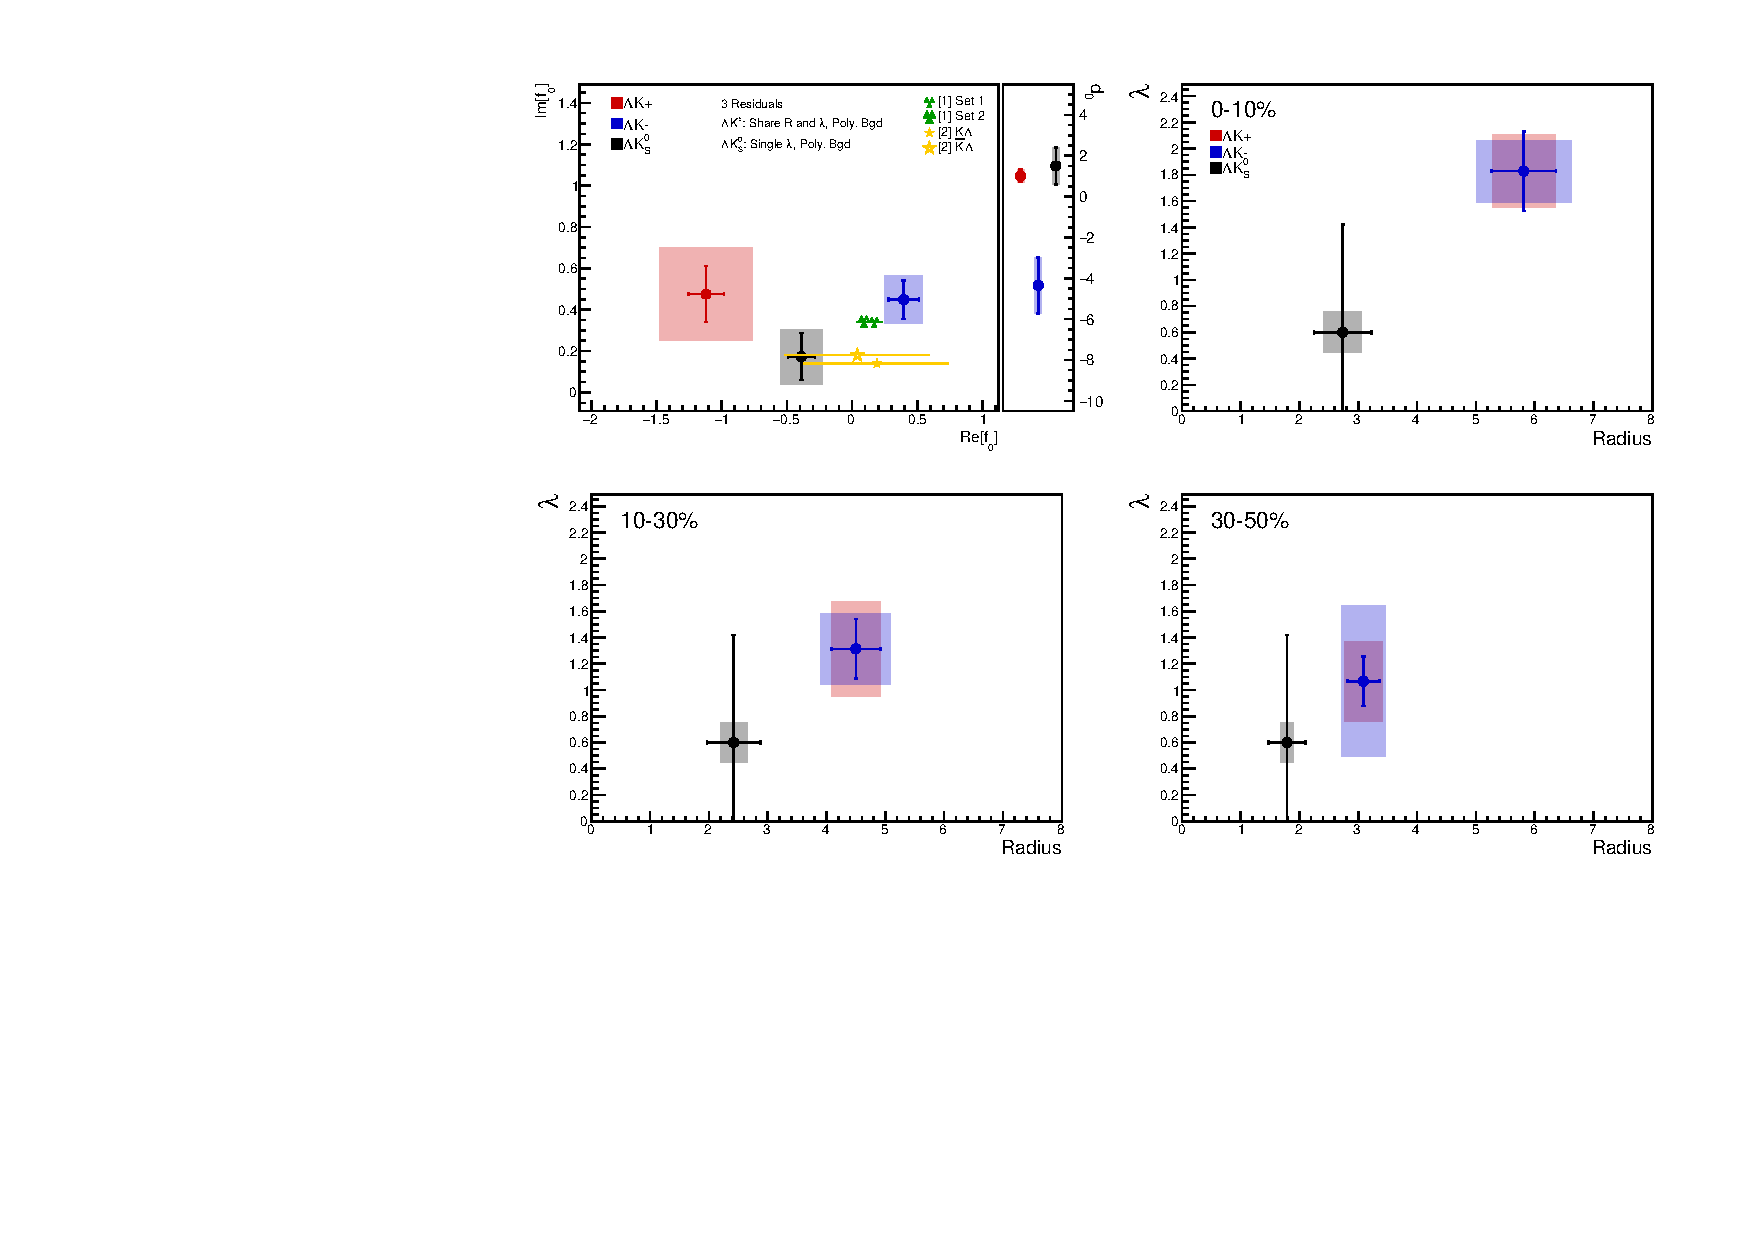
\includegraphics[width=0.80\textwidth]{7_ResultsAndDiscussion/Figures/CompareAllScattParams_Comp3An_3Res.pdf}
  \caption[Extracted Scattering Parameters: 3 Residuals in Fit]{Extracted scattering parameters for the case of 3 residual contributors for all of our $\Lambda$K systems.  [Top Left]: $\mathbb{I}f_{0}$ vs. $\mathbb{R}f_{0}$, together with d$_{0}$ to the right.  [Top Right (Bottom Left, Bottom Right)]: $\lambda$ vs. Radius for the 0-10\% (10-30\%, 30-50\%) bin.  The green \cite{Liu:2006xja} and yellow \cite{Mai:2009ce} points show theoretical predictions made using chiral perturbation theory.}
  \label{fig:ScattParams_Final}
\end{figure}

\clearpage

\subfile{7_ResultsAndDiscussion/7.1.1_ResultsLamK_NoRes.tex}
\subfile{7_ResultsAndDiscussion/7.1.2_ResultsLamK_3Res.tex}
\subfile{7_ResultsAndDiscussion/7.1.3_ResultsLamK_10Res.tex}
\subfile{7_ResultsAndDiscussion/7.1.4_ResultsLamK_FitMethodComparisons.tex}

\end{document}